% Possible types of documents/theses
%   doctype=bachelorsthesis
%   doctype=mastersthesis
%   doctype=idp
%   doctype=phdthesis
%   doctype=studienarbeit
%   doctype=diplomarbeit
%
% Document language
%   without 'lang' attribute: English
%   lang=ngerman:             German (new orthography)
%
% Binding correction
%   BCOR=<Längenangabe>
%   Additional margin, which is invisible due to binding the book
%   The usual binding by the Fachschaft has a thickness of 1,5 cm 
%
% biblatex (citations)
%   This requires 'biber' to be used instead of 'bibtex', please
%   adapt your editor's settings accordingly!
\documentclass[doctype=studienarbeit,lang=english,BCOR=15mm,biblatex]{ldvbook}
% Look for citation sources in the database "diplomarbeit.bib"
\addbibresource{diplomarbeit.bib}
\begin{document}

% Bibliographic information about the thesis, please change accordingly!
\title{Model Tuning and fair classification}
\author{Abdelrhman Abdelmooty, Ahmed Aziz Becheur, Rayen Dhahri,Bahaeddine Naili, Omar Tbeileh}
\license{CC-BY}



\maketitle[frontcover=Design1]




\tableofcontents



% Please compile this example document including the bibliography
% database. Check the resulting document and the references for 
% correct appearance (especially the German Umlaute).
% Thus you ensure that LaTeX is detecting the character encoding
% correctly and your build chain is working.
% If it does not, please tell your supervisor.



\chapter{Introduction}
\section{Project description}
This project aims to emphasize the concept of fairness in the context of machine intelligence and applies the learning outcomes and skills acquired within the course and the ability to interpret results based on a given dataset.
The main goal of this project is to be able to build a solid model that predicts a police stop outcome based on a set of features that  contains information about different individuals in the data set that some of them can be considered  sensitive, therefore might affect the model fairness. \\\\
\section{Methodology}
We basically used python 3 and some basic dependencies namely sklearn, pandas and numpy( a requirement.txt is provided with our project to have compatible full dependencies. Check the readme file for a guide of installation). To be able to work on the task, we created a private repository, where we kept track on the task’s distribution and the progress of the implementation.
To generate this report, we used the official latex template of the Chair for Data Processing that we worked on using overleaf. 

{\let\clearpage\relax\par \chapter{Implementation}}
\section{Data cleansing and encoding}
A first notice while starting to work on the dataset and inspecting it with 
df.head() 
df.dtypes()
is the fact that some columns were irrelevant as their attribute is static and can be dropping. The type of some columns made it a  necessary step to convert and encode some features as they were not numerical, thus not suitable for the training.\\
Before starting the encoding, we inspect the missing data. We noticed that for the drug\_related\_stop a lot of values were missing that covers 95\% the size of the column and cannot be treated with a custom .fillna(), so we dropped the feature. An additional reason for dropping this feature, is that after viewing some values we suspected that the column is high corrolated and discribed in the contrabound found, so we did a quick labelencoding and checked the corrolation through np.corrcoef(drug\_dum,contra) with both of them being the encoding of both columns with a high corrolation of 0.80 that confirms the doubt.
To make sure that all the remaining columns can be used, we checked for the corrolation between the remaining feautres then encoded the feature through a label encoder and keeping track on the encoding of the race \{1 :Black, 2 : Hispanic, 3 : Other, 4 : Asian\} and encoded the target manually so 1 which symbolize true is for the arrested and 0 for no action.

\section{Classification and performance measuring}
To predict, the stop outcome based on the available features, a simple k nearst neighbor (knn) Kneighborsclassifier was at first with arbitrary numbers of neighbors set to 5 implemented, this showed that Knn might be a good choice as classifier. \\
To implement a suitable KNeighborclassifier,  a parameter grid of different neighbors was set  and gridsearchcv was used to estimate the best number of neighbors for the classifier and had an accuracy of 0.944 and plotted the roc curve and the recall curve, as well as the auc score (0.959) to check for unbalanced classification and how good it performs. 
\begin{figure}[h]
    \centering
    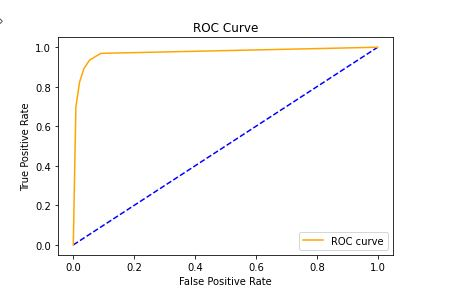
\includegraphics{roc.JPG}
    \caption[[width=1.0\textwidth,height=50]{Knn roc curve}
    \label{fig:knnl}
\end{figure}


The second classifier is a logistic regression that showed to be less accurate than the Kneighborclassifier that can be seen on the level of the roc curve and the accuracy of 0.81.
Compared to a dummy classifier that predicts all not arrested (the actual not arrested is 278273 making its accuracy around 0.692) both classifiers are still performing better. 

\section{Grouping features and fairness metrics}
For the rest of the implementations we pick the Kneighbourclassifier.
\begin{figure}[h]
    \centering
    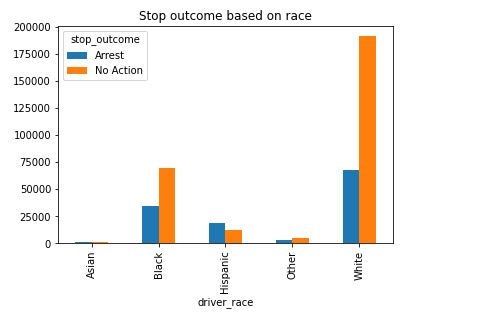
\includegraphics[width=10cm]{stopoutbased on race.JPG} 
    \label{fig:stop}%
\end{figure}
Looking into the dataset and the distribution of the ethnicities and their stop outcome added to the figure of the stop outcome based on race \ref{fig:stop} and the generated age figure (see src directory), we noticed that the training might be affected by these features. To confirm this behavior, races and another age-based groups were created, so by the end, we could study the behavior of the classification accordingly to  each case and to be able to detect possible discrimination. The age 30 shows a transformation point as after the “no action” rate increased enormously compared to the “Arrest" (The auto generated figure shows a high on arest and low on no action before and reversed after).
\begin{table}[h]
\centering
\begin{tabular}{lllll}
 Race& Age&  &  &  \\
 Black&  >=30&  &  &  \\
 Hispanic&  <30&  &  &  \\
 White&  &  &  & 
\end{tabular}
\caption{sensitive groups}
\end{table}


To avoid human error in the calculations, we made sure, which label after encoding belongs to which group, then we plotted the confusion matrixes of each group, we noticed that some groups like Hispanic ,black and people with the age <= 30 showed a higher false rate (false positives and false negatives). This showed an unbalance classification and a hint to the unfairness of the model. The hypothesis that the model is being “not fair” was confirmed once we called the separation,indepency and sufficiency of each group with their respective true positive, false positive, true negative,and false negative and calculated the difference that should have been as close to 0 as possible. 
This can be displayed as following: 
\begin{itemize}
    \item For hispanic: hispanic sep : (0.9401285583103764, 0.8836962294211365),
hispanic ind : 0.5911410270328955,
hispanic suf: (0.9211804930718013, 0.08921729611384784)
    \item for white : White sep :  (0.9122287464896605, 0.9582292653518215),
    White ind : 0.2522539927872231,
    White suf : (0.8804888866985363, 0.029974367469354304)
    \item we can as well display as an example the confusion matrix for the white group, the most frequent race to visualize the performance of the classifier (for other features check the notebook)
`\begin{figure}[h]
    \centering
    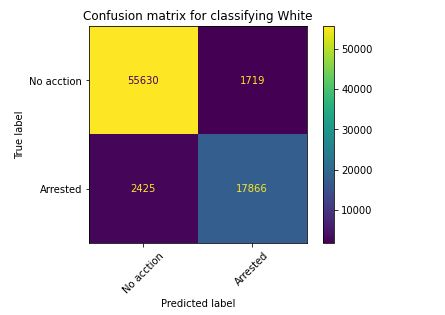
\includegraphics[width=8cm]{white.JPG}
    \caption[8cm]{confusion matrix for classifying white }
    \label{fig:whitebefore}
\end{figure}
\end{itemize}

\section{Excluding sensitive characteristics and retraining}
In this part we left  out of the model protected social attributes such as in our case driver race and age which are deemed as sensitive characteristics.\\  
While checking if our model is really fairer now after we dropout these sensitive features, we notice that our model performs better; we can observe the following example with the Hispanic-group before and after ignoring the driver race (see figure\ref{fig:my_label}).
\begin{figure}[h]
  
    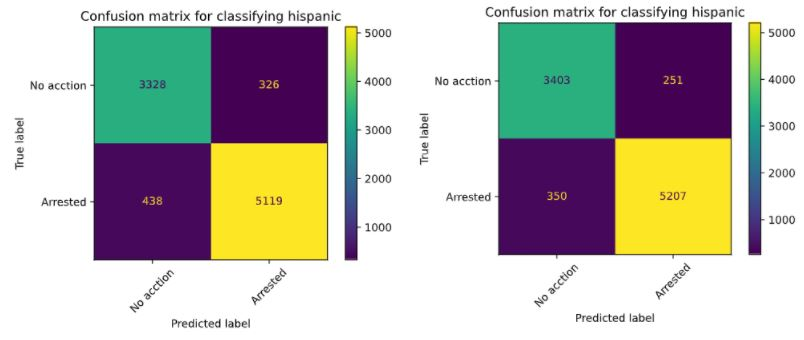
\includegraphics[width=0.98\columnwidth]{excluding.JPG}
    \caption{Hispanice confusion matrixes before and after feature exclusion}
    \label{fig:my_label}
\end{figure}
We can notice that the true negative and true positive values are much more better after ignoring the sensitive attribute, but,despite that, we can not assume that our model is now fairer than before.When Comparing some fairness criteria in regard to the same characteristics before and after we can judge that our model is not really improving in terms of fairness.
For the Hispanic-group the independence criterion remains the same (around 0.59) and by calculating the difference for the independence between the different groups from the race feature we can barely distinguish a difference, it is nearly the same\:(around 0.01).
	
Removing sensitive attributes does not erase the inequality but instead can perpetuate it.It may satisfy some criteria but not all of them.



$\longrightarrow$ Ignoring sensitive attributes altogether may not reveal these hidden correlations in data, this called redundant encoding.(No fairness through unawareness)
\section{Adapting thresholds for specific  groups}
As we have a very imbalanced dataset, this could lead to an unfair model which predicts labels based on a value that is highly present in the dataset. As we have investigated some features, it is remarkable that the driver race feature is based in the first place on White people (see figure \ref{fig:stop} a) and also has a very big difference between the two classes (Arrested/No\_Action).

This could force the model to set a very high percentage on white people to classify them as not arrested which is not fair. As it is represented in figure \ref{fig:whitebefore}, White people are often considered as non guilty when they actually are. The true negative value could be compromised and as a consequence, it could improve the accuracy of our model.
The method that we implemented to make the model fairer is to regroup the races into new groups to compromise the dominance of the white race with the less mentioned races in the dataset as the figure \ref{fig:stop} shows.
So we put White people and Other as a first subgroup and the rest (Black, Hispanic and Asian) as the second subgroup. 

In this case we will have in our dataset only two different races. With this new regroupment, we can see a very good improvement in our model based on the confusion matrix see \ref{fig:whitethresh}
\begin{figure}
    \centering
    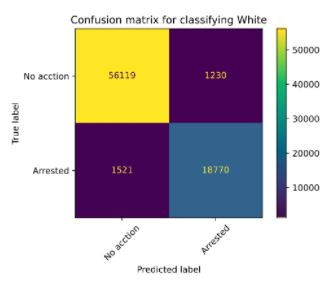
\includegraphics[width=6cm]{whiteafter.JPG}
    \caption{Confusion matrix for white after setting the threshold}
    \label{fig:whitethresh}
\end{figure} 
\begin{samepage}
One further method that we implemented to see if the model performs better, is to divide the age into an interval of ages. What is meant by this is to classify the driver's age by generation in this order 30 and above and younger than 30
The threshold as 30 years old represents the separation age between the peaks of being arrested or not according to the age (see generated figure as demensions are huge). So by setting this threshold the probability of being arrested would be high for people below 30 and lower for those above 30 years old (vice versa for No Action): the improvement can be viewed on the level of the new confusion matrices based on age (refer to the notebook). 
\let\clearpage\relax
\chapter{discussion and conclusion}
While working on the project, we recalled how Dressel and Farid \cite{pmid29376122} proved that a complex recidivism model like COMPASS is not significantly more accurate than the judgement of individuals with limited experience in criminal justice. They also argue that a predictor with two features is not necessarily inferior to the model with 137 features. This underlined to us the importance of communicating performance and assessing whether the level of accuracy a model has is appropriate to the application at hand.\\
To conclude, although our modifications enhanced the model’s performance for some groups, we believe it is irresponsible to deem this model fair. Not only because it is nearly a mathematical impossibility to tick all the boxes when it comes to fairness criteria (as proven by Larson.j  \cite{compass} and Sumpter \cite{ethics}), but also because there is no single superlative fairness metric to judge upon. It is also vital to remember that while this model only predicts an outcome without actually understanding what this outcome or its consequences are, the data behind it is a result of years of systematic discrimination. 
\end{samepage}



\printbibliography{}

\end{document}
